\documentclass[final,12pt,a4paper,oneside,article,danish]{memoir} %Her sættes document classen samt indstillinger for classen, her er den sat til at efterligne article. Her angives også om dokumentet er final eller draft. Angiv også sprog her.

%%%Tjek liste for brug af denne template
%%%%%%Indsæt forfatter istedet for Insert Author
%%%%%%Indsæt titel istedet for Insert Title
%%%%%%Vælg sprog ved babel, comment pakken dk-bib.
%%%%%%Vælg om der skal indholdsfortegnelse med ved at kommentere eller beholde de relevante linier: \tableofcontents
%%%%%%Vælg om der skal litteraturliste med ved at fjerne kommenttegn eller beholde dem: \bibliography
%%%%%%Husk at ændre draft til final når dokumentet er færdigt

%Specielle pakker for dansk support
\usepackage[utf8]{inputenc} %Her sørger jeg for at der er mulighed for at anvende danske bogstaver som æøå
\usepackage[danish]{babel} %Sørger for at ting som litteraturliste er på dansk. Husk at dansk support skal installeres fra MIKTEX settings
\renewcommand{\danishhyphenmins}{22} % bedre orddeling
\usepackage[T1]{fontenc} %Bedre support for europæiske accenterede tegn.
\linespread{1.1} %linjeafstanden stilles her

%Pakke der retter fejl i LaTeX kernen
\usepackage{fixltx2e}

%Set margin
\setlrmarginsandblock{2.5cm}{2.5cm}{*}
\setulmarginsandblock{2.5cm}{2.5cm}{*}


%Pakke for brug af anden font
\usepackage[sc]{mathpazo}
\usepackage{tgpagella}

%Pakker for opsætning af udseendet på siden
\nouppercaseheads %Sørger for at sidehoved er med små bogstaver

%Pakker der bruges i forbindelse med grafik og grafer
\usepackage[final]{graphicx} %Pakke som bruges til at inkludere grafik i dokumenterne
\graphicspath{{img/}}

%Tikz pakker til plotning, figurer og diagrammer
%\usepackage{pgfplots} %Bruges til at kunne plotte data på en graf i LaTeX, virker ikke med tikz-uml
%\pgfplotsset{compat=1.3} %Sætter pgfplots til at bruge ny standard med hensyn til placering af elementer.
\usepackage{xcolor} %Pakke der muligøre brugen af farver i pgfplots.
\usepackage{tikz} %Pakke til at plotte ting i LaTeX, se pgfmanual.pdf
\usetikzlibrary{positioning} %Bruges til bedre positionering af nodes.
\usetikzlibrary{intersections} %Bruges til at lave enhedscirklen.
\usetikzlibrary{calc}
\usepackage{tikz-uml} %Bruges til at tegne UML diagrammer i LaTeX

%Pakker der bruges i forbindelse med tabeller
\usepackage{booktabs} %Benyttes til at lave bedre horisontale linjer i tabeller.
\usepackage{dcolumn} %Benyttes til at lave tabelkolonner, hvor decimaladskilleren bruges til at aligne.
\newcolumntype{d}[1]{D{.}{.}{#1}} %Laver en ny column type som er den der oftest bruges i dette projekt.
\newcommand\mc[1]{\multicolumn{1}{c}{#1}} %Giver kommandoen mc{tekst} som bruges til at sørge for at teksten i dcolumn kolonner ikke bliver formateret som matematik.
\usepackage{multirow} %Giver mulighed for celler der strækker sig over flere rækker.
\renewcommand\multirowsetup{\centering} %Sikre at alt der skrives i multirow er centreret.
\usepackage{bigstrut}

%Pakker til brug for matematik samt diverse symboler
\usepackage{amsmath} %Til brug for matematik.
\usepackage{amsfonts}
\usepackage{amssymb}
\usepackage{sistyle} %Se side 263 Introduktion til Latex giver mulighed for \SI{nummer}{enhed} kommandoen, som sørger for at enhederne og tallene er stillet rigtigt op.
\SIstyle{German} %Sætter stylen for enheder og numre til tysk.
\usepackage{textcomp} %Ekstra symboler

%Pakker som ordner nummereringen af formler og figurer Disse kommer fra amsmath
\numberwithin{equation}{chapter} %For at få sektions numre på formler til henvisninger.
\numberwithin{figure}{chapter} %For at få sektions numre på figure til henvisninger.
\numberwithin{table}{chapter} %For at få sektions numre på tabeller til henvisninger.
\usepackage{placeins} %Kan bruges til at stoppe floats fra at passerer sections

%Make sure all figures are placed with htbp
\makeatletter
\renewcommand\fps@figure{htbp} %Sørger for at alle figurer bliver placeret i forhold til htbp.
\renewcommand\fps@table{htbp} %Sørger for at alle tabeller bliver placeret i forhold til htbp.
\g@addto@macro{\quote}{\itshape} %Laver tekst i quote environmentet kursiv.
\makeatother

%Misc
%\usepackage[final]{pdfpages} %Enables insertion of external multipage pdf files.

%Pakker som kan bruges til at angives hvor langt ned LaTeX skal nummere sektioner%%%
\setsecnumdepth{subsection} % Nummerering ned til subsection hvis den sættes til subsection

%Pakker der bruges til litteraturlister%%%
\usepackage[backend=biber,style=alphabetic]{biblatex} 

%Pakker der bruges til at lave referencer i dokumentet
\usepackage{prettyref}
\usepackage[danish]{varioref} %Giver adgang til kommandoen \vref som giver nummer og sidehenvisning > 0.1 på side 4

%Pakker der bruges for at lave klikbare links i pdf filer
\usepackage[pdftex, colorlinks=false, pdfauthor={Gruppe 21}, pdftitle={CDIO del 2}]{hyperref} %EDIT Til hyperlinks i dokumentet [colorlinks] kan tilføjes for farver, klikbare links i pdf filerne. citecolor=black
\usepackage{memhfixc} %Løser problemer med hyperref i memoir, skal loades efter hyperref.

%Pakker der bruges for at sikre at der bruges de korrekte kvotationstegn
\usepackage[danish=quotes]{csquotes} %gør det muligt at bruge \enquote{quote} se evt s. 25 i Introduktion til Latex ellers kan "` quote "' bruges. Dansk indstilling [danish=quotes].

%Pakke der bruges til at lave noter til mig selv i draft
\usepackage[danish]{fixme} %pakke der bliver brugt til at lave noter til mig selv om ting der skal rettes. \fxfatal, \fxerror, \fxwarning, \fxnote[inline]{text}. Om dokumentet er draft eller final angives ved \documentclass.

%Indstillinger af caption
\captionnamefont{\footnotesize\bfseries}
\captiontitlefont{\footnotesize\itshape}
%\setsecheadstyle{\bfseries\large\itshape}

%Sidehoved og -fod herunder
\makeatletter
\makepagestyle{bachstyle}
\makeoddhead{bachstyle}{\small \leftmark}{}{\small CDIO del 2}
\makeoddfoot{bachstyle}{}{}{\small\thepage}
\makepsmarks {bachstyle}{
\createmark{chapter}{both} {shownumber} {\@chapapp\ }{. \ }
\createmark{section} {right}{nonumber} {} {. \ }
\createmark{subsection} {right}{nonumber} {} {. \ }
\createmark{subsubsection}{right}{nonumber} {} {. \ }
\createplainmark{toc} {both}{\contentsname}
\createplainmark{lof} {both}{\listfigurename}
\createplainmark{lot} {both}{\listtablename}
\createplainmark{bib} {both}{\bibname}
\createplainmark{index} {both}{\indexname}
}
\nouppercaseheads % ingen rene kapitaler
\makeatother
\copypagestyle{plain}{bachstyle}
\makeevenhead{plain}{}{}{} % slet venstre sidehoved
\makeoddhead{plain}{}{}{}% slet højre sidehoved

%Giver kommandoer for at bruge \Re og \Im til komplekse tal.
\renewcommand{\Re}{\operatorname{Re}}
\renewcommand{\Im}{\operatorname{Im}}

\newcommand{\iv}[1]{\paragraph{#1}\fancybreak{}}
\usepackage{soul}
\sodef\an{}{0.2em}{.9em plus.6em}{1em plus.1em minus.1em}
\newcommand\stext[1]{\an{\scshape#1}}

%Nye kommandoer til kode
\newcommand{\codeparagraph}[1]{\paragraph{\texttt{#1}}}
\newcommand{\klasse}[1]{\texttt{\textit{#1}}}
\newcommand{\metode}[1]{\texttt{#1}}

%Memoir checkandfixthelayout
\checkandfixthelayout[nearest] 

%Choosing the bibliography to load
\bibliography{main}

\begin{document} %Dokumentet begynder herunder 
\pagestyle{bachstyle}
\author{Gruppe 21} %EDIT Her sættes dokumentets forfatter
\title{CDIO del 2} %EDIT Her sættes dokumentets titel
%Titelside begynder
%\maketitle
%\thispagestyle{empty}
%\newpage
\noindent {\large\bfseries Projektopgave efterår 2012 - jan 2013}

\noindent {\large\bfseries 02312-14 Indledende programmering og 02313 Udviklingsmetoder til IT-Systemer.}
{\normalsize

\noindent Projekt navn: del2

\noindent Gruppe nr: 21.

\noindent Afleveringsfrist: Mandag den 12/11-2012 kl. 05:00

\noindent Denne rapport er afleveret via Campusnet (der skrives ikke under)

\noindent Denne rapport indeholder 23 sider incl. denne side.
}
\fancybreak{}
\noindent \emph{Studie nr, Efternavn, Fornavne}
\fancybreak{}

\noindent s122996, Caspersen, Martin

\noindent Kontakt person (Projektleder)

\noindent 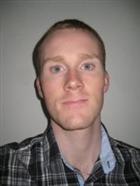
\includegraphics[width=2cm]{martin.jpg}

\noindent s100182, Baltzersen, Jesper Engholm

\noindent 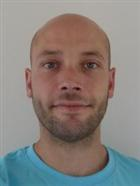
\includegraphics[width=2cm]{jesper.jpg}
\newpage
% Table generated by Excel2LaTeX from sheet 'Timeregnskab'
\begin{table}[htbp]
  \centering
    \begin{tabular}{|l|l|r|r|r|r|r|r|}
    \hline
    CDIO del 3 &       &       &       &       &       &       &  \bigstrut\\
    \hline
    Time-regnskab & Ver. 2012-11-30 &       &       &       &       &       &  \bigstrut\\
    \hline
          &       &       &       &       &       &       &  \bigstrut\\
    \hline
    Dato  & Deltager & Design & Impl. & Test  & Dok.  & Andet & Ialt \bigstrut\\
    \hline
    2012-11-13 & Martin &       & 2     &       &       &       & 2 \bigstrut\\
    \hline
    2012-11-20 & Martin &       & 5     &       &       &       & 5 \bigstrut\\
    \hline
    2012-11-20 & Jesper &       & 5     &       &       &       & 5 \bigstrut\\
    \hline
    2012-11-23 & Martin & 2     &       &       & 2     &       & 4 \bigstrut\\
    \hline
    2012-11-23 & Jesper &       &       &       & 2     &       & 2 \bigstrut\\
    \hline
    2012-11-24 & Martin &       &       &       & 5     &       & 5 \bigstrut\\
    \hline
    2012-11-27 & Jesper &       &       &       & 5     &       & 5 \bigstrut\\
    \hline
    2012-11-27 & Martin &       &       &       & 3     &       & 3 \bigstrut\\
    \hline
    2012-11-28 & Martin &       &       &       & 2     &       & 2 \bigstrut\\
    \hline
    2012-11-29 & Jesper &       &       &       & 2     &       & 2 \bigstrut\\
    \hline
    2012-11-30 & Jesper &       &       &       & 3     &       & 3 \bigstrut\\
    \hline
    2012-11-30 & Martin &       &       &       & 4     &       & 4 \bigstrut\\
    \hline
          & Sum   & 2     & 12    & 0     & 28    & 0     & 42 \bigstrut\\
    \hline
    \end{tabular}%
  \label{tab:addlabel}%
\end{table}%

%Abstract begynder
%\mainmatter
%SLETTET\input{abstract.tex}
%Abstract slutter
%Titelside slutter
%Indholdsfortegnelse begynder
\newpage
%\thispagestyle{empty}
\FloatBarrier
\tableofcontents
%\thispagestyle{empty}
\newpage
%Indholdsfortegnelse slutter
%%%Herunder begynder selve indholdet%%%
\chapter{Indledning[1]}\label{chap:indledning}
Denne rapport er udarbejdet i kurserne 02313 Udviklingsmetoder til IT-systemer, 02312 Indledende programmering på første semester af Diplomigneniør IT. Opgaven er del tre af tre CDIO opgaver på første semester, det overordnede formål med opgaverne på semesteret er at lave et Matador spil. Denne tredje opgave fokuserer på at implementere et klassehieraki over felterne i et matadorspil og modificere spillet fra del 2. Den nærmere kravspecificering til opgaven findes i "CDIO\_opgave\_del3.pdf"\cite{CDIOdel3}, kravene bliver behandlet i \vref{chap:krav}. Opgaven bygger på undervisning modtaget i ovenstående kurser hvor der blev benyttet bøgerne \cite{umlbook} og \cite{javabook}. Igennem opgaverne vil klasser blive vist på følgende måde \klasse{KlasseNavn}, metoder \metode{metodeNavn()} og design patterns \dpattern{DesignPattern}.

Rapporten er sat med \LaTeX, UML diagrammer er lavet med Ti\emph{k}Z-UML og andre figurer er lavet med Ti\emph{k}Z og \textsc{PGF}.

Bemærk venligst at Martin Caspersen tidligere var med i gruppe 14 og Jesper Engholm Baltzersen tidligere var med i gruppe 17. Begge skrev størstedelen af rapporterne til CDIO del 1 og derfor kan der forekomme passager i denne rapport som minder om passager fra gruppe 14 og 17s rapporter til CDIO del 1. Kodebasen der er benyttet som udgangspunkt for del 2 er den kode som Gruppe 14 afleverede til del 1.

\section{Ansvarfordeling}\label{sec:indledning:ansvarsfordeling}

Ansvarsfordelingen i opgaven er anført i overskrifterne til de forskellige afsnit og benytter følgende numre for at beskrive gruppens medlemmer:
\begin{enumerate}
\item Martin Caspersen
\item Jesper Engholm Baltzersen
\end{enumerate}
Ansvarsfordelingen overskues nemmest i indholdsfortegnelsen. Hvis der er nummer på et af hovedafsnittene og ikke nogen numre på underafsnit er det pågældende medlem ansvarlig for alle underafsnittene også.

Alle figurer og diagrammerne er udarbejdet af Martin, men både Martin og Jesper er ansvarlige for indholdet af disse.

Ansvaret for kodningen af de forskellige klasser er beskrevet herunder:
\begin{itemize}
\item Die [1, 2]
\item MatadorRafleBaeger [1, 2]
\item Game [1, 2]
\item Player [1, 2]
\item BoundaryToGUI [1, 2]
\item BoundaryToPlayer [1, 2]
\item Main [1, 2]
\item Board [1, 2]
\item Field og underklasser [1, 2]
\item TestDie [1, 2]
\end{itemize}
\newpage
%Slut af indholdet
%Herunder hentes litteraturlisten fra bib filen, kun de poster der bliver citeret bliver vist
\printbibliography
%Litteraturliste slut
\listoffixmes %liste af rettelser fra fixme
%Herunder er slutningen af dokumentet
\end{document}